\documentclass[../../main.tex]{subfiles}
\graphicspath{{\subfix{../../image/}}} % 指定图片目录,后续可以直接使用图片文件名。

% 例如:
% \begin{figure}[h]
% \centering
% \includegraphics{image-01.01}
% \label{fig:image-01.01}
% \caption{图片标题}
% \end{figure}

\begin{document}

\section{群}

\begin{definition}
令 $(S, \cdot)$ 是一个幺半群,$x \in S$。我们称 $x$ 是\textbf{可逆的},当且仅当
\begin{align*}
\exists y \in S, x \cdot y = y \cdot x = e
\end{align*}
其中 $y$ 被称为 $x$ 的\textbf{逆元},记作 $x^{-1}$。 
\end{definition}

\begin{proposition}[逆元存在必唯一]
令 $(S, \cdot)$ 是一个幺半群。假设 $x \in S$ 是可逆的,则其逆元唯一。也就是说,如果 $y, y' \in S$ 都是它的逆元,则 $y = y'$。
\end{proposition}
\begin{proof}
假设 $y, y'$ 都是 $x$ 的逆元。则 $y \cdot x = e$,$x \cdot y' = e$.从而
\begin{align*}
y = y \cdot e = y \cdot x \cdot y' = e \cdot y' = y' .
\end{align*}
\end{proof}

\begin{definition}[群]
令 $(G, \cdot)$ 是一个幺半群,若$G$ 中所有元素都是可逆的,则我们称$(G,\cdot)$是一个\textbf{群}.换言之,若 $\cdot$ 是 $G$ 上的一个二元运算,则我们称 $(G, \cdot)$ 是个\textbf{群},或 $G$ 对 $\cdot$ 构成群,当这个运算满足结合律,存在单位元,且每个元素具有逆元。再进一步展开来说,同样等价地,若 $\cdot$ 是 $G$ 上的一个二元运算,则我们称 $(G, \cdot)$ 是个\textbf{群},当
\begin{gather*}
\forall x, y, z \in G, x \cdot (y \cdot z) = (x \cdot y) \cdot z ,\\
\exists e \in G, \forall x \in G, x \cdot e = e \cdot x = x ,\\
\forall x \in G, \exists y \in G, x \cdot y = y \cdot x = e .
\end{gather*} 
\end{definition}

\begin{proposition}
令 $(G, \cdot)$ 是一个群,令 $x \in G$,则 $(x^{-1})^{-1} = x$。
\end{proposition}
\begin{proof}
方便起见,我们令 $y = x^{-1}$,于是有 $x \cdot y = y \cdot x = e$。我们要证明 $y^{-1} = x$,而这就是 $y \cdot x = x \cdot y = e$,显然成立。这就证明了逆元的逆元是自身.
\end{proof}

\begin{proposition}
令 $(G, \cdot)$ 是一个群,令 $x, y \in G$,则 $(x \cdot y)^{-1} = y^{-1} \cdot x^{-1}$。
\end{proposition}
\begin{proof}
我们利用定义来证明。一方面,利用广义结合律,$(x \cdot y) \cdot (y^{-1} \cdot x^{-1}) = e$;另一方面,同理可以得到另一边的等式$(y^{-1} \cdot x^{-1}) \cdot (x \cdot y) = e$,这就告诉我们 $(x \cdot y)^{-1} = y^{-1} \cdot x^{-1}$。 
\end{proof}

\begin{definition}[Abel群]
若 $(G, \cdot)$ 是一个群,我们称它是\textbf{Abel群},或\textbf{交换群},当该运算满足交换律,即
\begin{align*}
\forall x, y \in G, x \cdot y = y \cdot x
\end{align*} 
\end{definition}

\begin{example}[$\,\,$常见的群]
\begin{enumerate}
\item 我们称只有一个元素的群为\textbf{平凡群},记作${e}$.其中的二元运算是$e\cdot e=e$.
\item 常见的加法群有$(\mathbb{Z},+),$ $(\mathbb{Q},+),$ $(\mathbb{R},+),$ $(\mathbb{C},+)$等.这些加法群分别称为整数加群、有理数加群、实数加群、复数加群.
\item 常见的乘法群有$(\mathbb{Q}^\times,+),$ $(\mathbb{R}^\times,+),$ $(\mathbb{C}^\times,+)$等, 其中$\mathbb{Q}^\times=\mathbb{Q}\backslash {0}$,类似地定义其余两个集合.这些乘法群分别称为有理数乘群、实数乘群、复数称群.
\item 在向量空间中,$n$维欧式空间对加法构成群即$(\mathbb{R}^n,+)$.类似地$(\mathbb{C}^n,+),$ $(\mathbb{Q}^n,+),$ $(\mathbb{Z}^n,+)$也是群.对于这些群,单位元都是零向量,加法逆元则是对每个坐标取相反数,如$(x_1,\cdots,x_n)$的加法逆元是$(-x_1,\cdots,-x_n)$.
\item 所有的$m\times n$矩阵也对加法构成群,单位元都是零矩阵,加法逆元则是对每一项取相反数.对于$n\times n$的实矩阵加法群,我们记作$(M(n,\mathbb{R}),+)$,类似地我们将$n\times n$的复矩阵加法群记作$(M(n,\mathbb{C}),+)$.
\end{enumerate}
\end{example}
\begin{proof}
证明都是显然的.
\end{proof}

\begin{lemma}
令 $(S, \cdot)$ 是一个幺半群,令 $G$ 是其所有可逆元素构成的子集,则 $(G, \cdot)$ 是个群。
\end{lemma}
\begin{remark}
我们称呼幺半群中的可逆元素为 “\textbf{单位}”,因此 $G$ 是由所有该运算下的单位构成的集合(在这里甚至是群)。
\end{remark}
\begin{proof}
首先结合律完全继承自 $S$,不需要证明。而单位元是可逆的,因此 $e \in G$。剩下要证明 $G$ 中每个元素都有($G$ 中的)逆元,而这几乎是显然的。假设 $x \in G$,则 $x$ 是可逆元素,我们取 $y \in S$,使得 $x \cdot y = y \cdot x = e$(这里要注意我们只能首先保证 $y$ 在全集 $S$ 中)。接下来我们要证明 $y \in G$,即 $y$ 可逆,而这是显然的,因为 $x$ 正是它的逆。所以 $y \in G$。这样,就证明了 $(G, \cdot)$ 是个群.
\end{proof}

\begin{definition}[子群]
令 $(G, \cdot)$ 是一个群,且 $H \subset G$。我们称 $H$ 是 $G$ 的\textbf{子群},记作 $H < G$,当其包含了单位元,在乘法和逆运算下都封闭,即
\begin{gather*}
e \in H ,\\
\forall x, y \in H, x \cdot y \in H ,\\
\forall x \in H, x^{-1} \in H.
\end{gather*} 
\end{definition}

\begin{proposition}[子群也是群]
令 $(G, \cdot)$ 是一个群。若 $H$ 是 $G$ 的子群,则 $(H, \cdot)$ 也是个群。
\end{proposition}
\begin{proof}
就二元运算的良定义性而言,子群第一个条件(封闭性)就满足了,这使得我们后面的谈论是有意义的。首先,结合律肯定满足,因为它是个子集。其次,根据子群的第二个条件,$e \in H$ 是显然的。再次,我们要证明每个 $H$ 中元素有 $H$ 中的逆元,而这是子群的第三个条件。
\end{proof}

\begin{proposition}[子群的等价条件]\label{proposition:子群的等价条件}
$(H,\cdot)$是子群等价于
\begin{gather*}
e \in H,\\
\forall x, y \in H, x \cdot y^{-1} \in H .
\end{gather*}
\end{proposition}
\begin{proof}
假设$(H,\cdot)$是子群。令 $x, y \in H$,利用逆元封闭性得到 $y^{-1} \in H$,再利用乘法封闭性得到 $x \cdot y^{-1} \in H$。

反过来,假设上述条件成立.令 $x \in H$,则 $e \cdot x^{-1} = x^{-1} \in H$,这证明了逆元封闭性。
接下来,令 $x, y \in H$,则利用逆元封闭性,$y^{-1} \in H$,故 $x \cdot (y^{-1})^{-1} = x \cdot y \in H$。这就证明了乘法封闭性。

综上,这的确是子群的等价条件。
\end{proof}

\begin{definition}[一般线性群]
我们对于那些 $n*n$ 可逆实矩阵构成的乘法群,称为\textbf{(实数上的)$n$ 阶一般线性群},记作 $(GL(n, \mathbb{R}), \cdot)$。由于一个矩阵可逆当且仅当其行列式不为零,因此
\begin{align*}
GL(n, \mathbb{R}) = \{A \in M(n, \mathbb{R}) : \det(A) \neq 0\}.
\end{align*} 
\end{definition}

\begin{definition}[特殊线性群]
我们将由那些行列式恰好是 $1$ 的 $n*n$ 实矩阵构成的乘法群称为\textbf{(实数上的)$n$ 阶特殊线性群},记作 $(SL(n, \mathbb{R}), \cdot)$,即
\begin{align*}
SL(n, \mathbb{R}) = \{A \in M(n, \mathbb{R}) : \det(A) = 1\}.
\end{align*} 
\end{definition}

\begin{proposition}
$(SL(n, \mathbb{R}), \cdot)$ 是个群。
\end{proposition}
\begin{proof}
根据定义,$SL(n, \mathbb{R})$ 首先是 $GL(n, \mathbb{R})$ 的子集,那么只要证明它是个子群即可。首先,乘法单位元单位矩阵的行列式恰好是 1(这也是为什么我们定义特殊线性群是行列式是 1 的矩阵构成的群的原因),这就证明了 $I \in SL(n, \mathbb{R})$($I = I_n$ 指的是 $n$ 阶单位矩阵)。另外,我们要证明 $SL(n, \mathbb{R})$ 在乘法下封闭。令 $A, B$ 是两个行列式为 1 的 $n*n$ 实矩阵。由于行列式满足 $\det(AB) = \det(A)\det(B)$,因此 $AB$ 的行列式也是 1,也就在特殊线性群中。这就证明了特殊线性群确实是个群。至于逆元封闭性,我们利用 $\det(A^{-1}) = \frac{1}{\det(A)}$。假设 $\det(A) = 1$,则 $\det(A^{-1}) = 1$,于是 $A^{-1} \in SL(n, \mathbb{R})$。综上,特殊线性群确实是个群。 
\end{proof}

\begin{definition}[群同态]
令 $(G, \cdot), (G', *)$ 是两个群,且 $f : G \to G'$ 是一个映射。我们称 $f$ 是一个\textbf{群同态},当其保持了乘法运算,即
\begin{align*}
\forall x, y \in G, f(x \cdot y) = f(x) * f(y).
\end{align*} 
\end{definition}

\begin{proposition}
若 $f : (G, \cdot) \to (G', *)$ 是一个群同态,则 $f(e) = e'$,$f(x^{-1}) = f(x)^{-1}$。
\end{proposition}
\begin{note}
也就是说,$f$ 不仅把乘积映到乘积,而且把单位元映到单位元,把逆元映到逆元。在这个意义下,实际上 $f$ 将所有群 $G$ 的 “信息” 都保持到了 $G'$ 上,包括单位元,乘法和逆元。至于结合律(或者更基础的封闭性),显然两边本来就有,就不必再提。
\end{note}
\begin{proof}
首先,因为 $e \cdot e = e$,所以利用同态的性质,$f(e) = f(e \cdot e) = f(e) * f(e)$。这时,两边同时左乘 $f(e)^{-1}$,就可以各约掉一个 $f(e)$,得到 $e' = f(e)$,这就证明了 $f$ 把单位元映到单位元。

另一方面,令 $x \in G$,则 $e' = f(e) = f(x \cdot x^{-1}) = f(x) * f(x^{-1})$。同理 $e' = f(x^{-1}) * f(x)$。于是由定义,$f(x^{-1})$ 就是 $f(x)$ 的逆元,即 $f(x^{-1}) = f(x)^{-1}$。这就证明了这个命题。 
\end{proof}

\begin{proposition}
$\det : GL(n, \mathbb{R}) \to (\mathbb{R}^\times, \cdot)$ 是一个乘法群同态。 
\end{proposition}
\begin{proof}
证明都是显然的.
\end{proof}

\begin{definition}[群同态的核与像]
令 $f : (G, \cdot) \to (G', *)$ 是一个群同态,则我们定义 $f$ 的\textbf{核}与\textbf{像},记作 $\ker(f)$ 与 $\mathrm{im}(f)$,分别为
\begin{align*}
\ker(f) &= \{x \in G : f(x) = e'\} \subset G \\
\mathrm{im}(f) &= \{y \in G' : \exists x \in G, y = f(x)\} = \{f(x) : x \in G\} \subset G'
\end{align*} 
\end{definition}

\begin{figure}[htbp]
\centering
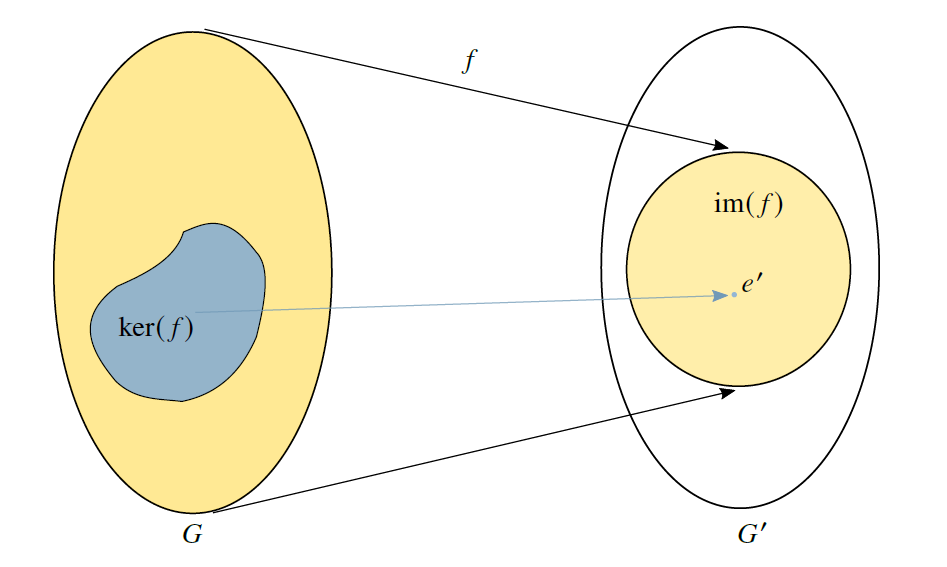
\includegraphics[scale=0.5]{群同态的核与像示意图.png}
\label{figure:群同态的核与像示意图}
\caption{群同态的核与像示意图}
\end{figure}








\end{document}